\begin{frame}{Learning Rate}
    \begin{itemize}
        \item Learning rate is a hyper-parameter that controls how much we are adjusting the weights of our network with respect the loss gradient. 
        \begin{figure}[H]
    		\centering
    		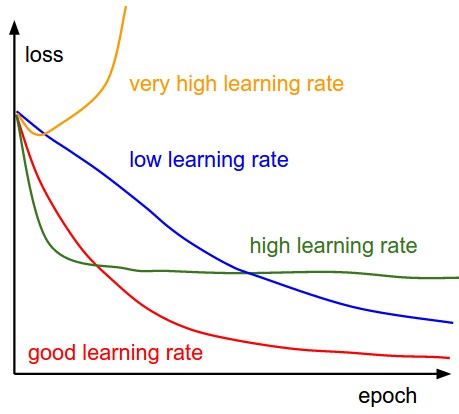
\includegraphics[width=0.5\textwidth]{Images/lr.png}
    		\caption{Learning Rate Effect}
	    \end{figure}
	    \item The lower the value of learning rate, the slower we travel along the downward slope.
	    \item While this might be a good idea (using a low learning rate) in terms of making sure that we do not miss any local minima, it could also mean that we’ll be taking a long time to converge
    \end{itemize}        
\end{frame}


\begin{frame}{Vanishing/Exploding Gradient}
    \begin{itemize}
        \item Exploding
        \begin{itemize}
            \item In a network of n hidden layers, n derivatives will be multiplied together.
            \item If the derivatives are large then the gradient will increase exponentially as we propagate down the model until they eventually explode.
            \item If the gradients keep on getting larger and larger as the backpropagation algorithm progresses. 
            \item This, in turn, causes very large weight updates and causes the gradient descent to diverge. 
        \end{itemize}
        \item Vanishing
        \begin{itemize}
            \item The derivatives are smaller then the gradient
            \item It will decrease exponentially as we propagate through the model until it eventually vanishes,
            \item As the backpropagation algorithm advances downwards(or backward) from the output layer towards the input layer, the gradients often get smaller and approach zero which eventually leaves the weights of the initial or lower layers nearly unchanged.
            \item As a result, the gradient descent never converges to the optimum. 
        \end{itemize}
    \end{itemize}
\end{frame}

\begin{frame}{Vanishing/Exploding Gradient Reasons}
    \begin{itemize}
        \item Exploding
        \begin{itemize}
            \item The model is not learning much on the training data therefore resulting in a poor loss.
            \item The model will have large changes in loss on each update due to the models instability.
        \end{itemize}
        \item Vanishing
        \begin{itemize}
            \item The model will improve very slowly during the training phase and it is also possible that training stops very early, meaning that any further training does not improve the model.
            \item The weights closer to the output layer of the model would witness more of a change whereas the layers that occur closer to the input layer would not change much (if at all).
            \item Model weights shrink exponentially and become very small when training the model.
        \end{itemize}
    \end{itemize}
\end{frame}

\begin{frame}{Vanishing/Exploding Gradient Solutions}
    \begin{itemize}
        \item Proper Weight Initialization 
        \begin{itemize}
            \item The variance of outputs of each layer should be equal to the variance of its inputs.
            \item The gradients should have equal variance before and after flowing through a layer in the reverse direction.
        \end{itemize}
        \item Batch Normalization
        \begin{itemize}
            \item It consists of adding an operation in the model just before or after the activation function of each hidden layer.
            \item This operation simply zero-centers and normalizes each input, then scales and shifts the result using two new parameter vectors per layer: one for scaling, the other for shifting.
            \item In other words, the operation lets the model learn the optimal scale and mean of each of the layer’s inputs.
            \item To zero-center and normalize the inputs, the algorithm needs to estimate each input’s mean and standard deviation.
            \item It does so by evaluating the mean and standard deviation of the input over the current mini-batch (hence the name “Batch Normalization”).
        \end{itemize}
    \end{itemize}
\end{frame}

\begin{frame}{Saturating Functions}
    \begin{itemize}
        \item Intuition
        \begin{itemize}
            \item A saturating activation function squeezes the input.
        \end{itemize}
        \item Definition
        
        \item Examples
        \begin{itemize}
            \item The tanh (hyperbolic tangent) activation function is saturating as it squashes real numbers to range between (0, 1)
            \item The sigmoid activation function is also saturating, because it squashes real numbers to range between (0, 1).
            \item In contrast, The Rectified Linear Unit (ReLU) activation function is non-saturating.
        \end{itemize}
    \end{itemize}
    
\end{frame}